\let\negmedspace\undefined
\let\negthickspace\undefined
\documentclass[journal]{IEEEtran}
\usepackage[a5paper, margin=10mm, onecolumn]{geometry}
%\usepackage{lmodern} % Ensure lmodern is loaded for pdflatex
\usepackage{tfrupee} % Include tfrupee package

\setlength{\headheight}{1cm} % Set the height of the header box
\setlength{\headsep}{0mm}     % Set the distance between the header box and the top of the text

\usepackage{gvv-book}
\usepackage{gvv}
\usepackage{cite}
\usepackage{amsmath,amssymb,amsfonts,amsthm}
\usepackage{algorithmic}
\usepackage{graphicx}
\usepackage{textcomp}
\usepackage{xcolor}
\usepackage{txfonts}
\usepackage{listings}
\usepackage{enumitem}
\usepackage{mathtools}
\usepackage{gensymb}
\usepackage{comment}
\usepackage[breaklinks=true]{hyperref}
\usepackage{tkz-euclide} 
\usepackage{listings}
% \usepackage{gvv}                                        
\def\inputGnumericTable{}                                 
\usepackage[latin1]{inputenc}                                
\usepackage{color}                                            
\usepackage{array}                                            
\usepackage{longtable}                                       
\usepackage{calc}                                             
\usepackage{multirow}                                         
\usepackage{hhline}                                           
\usepackage{ifthen}                                           
\usepackage{lscape}
\begin{document}

\bibliographystyle{IEEEtran}
\vspace{3cm}

\title{1-1.10-21}
\author{AI24BTECH11015 - Harshvardhan Patidar}
 \maketitle
% \newpage
% \bigskip
{\let\newpage\relax\maketitle}

\renewcommand{\thefigure}{\theenumi}
\renewcommand{\thetable}{\theenumi}
\setlength{\intextsep}{10pt} % Space between text and floats


\numberwithin{equation}{enumi}
\numberwithin{figure}{enumi}
\renewcommand{\thetable}{\theenumi}

Question: \\
	Write down a unit vector in $XY$-plane, making an angle of $30^{\degree}$ with the positive direction of $X$ axis. \\ \\

\solution: \\
		\begin{table}[h!]    
  			\centering
  			\begin{tabular}[12pt]{ |c| c|}
    \hline
    \textbf{Variable} & \textbf{Description}\\
    \hline
	$\vec{m}$ & Unit Vector\\
    \hline
	$\alpha$ & Angle of the unit vector with $x$-axis\\
    \hline
	$\beta$ & Angle of the unit vector with $y$-axis\\
    \hline	
    \end{tabular}

  			\caption{Variables Used}
  			\label{tab1-1.10-21}
		\end{table}\\


	We have, in the $2$-D space, the unit direction vector is given by
	\begin{align}
		\vec{m} &= \myvec{\cos \alpha \\ \cos \beta}
	\end{align}

	Given, 
	\begin{align}
		\alpha &= 30^{\degree} \label{eqn1}
	\end{align}

	So,
	\begin{align}
		\beta &= 90^{\degree} - \alpha\\
		\beta &= 60^{\degree}
	\end{align}

	Putting values in \eqref{eqn1}, we get
	\begin{align}
		\vec{m} &= \myvec{\cos 30^{\degree} \\ \cos 60^{\degree}}\\
		\vec{m} &= \myvec{\frac{\sqrt{3}}{2} \\ \frac{1}{2}}\\	
	\end{align}

	So,
	\begin{align}
		\vec{m} &= \frac{1}{2} \myvec{\sqrt{3} \\ 1}
	\end{align}


	\begin{figure}[H]
		\centering
		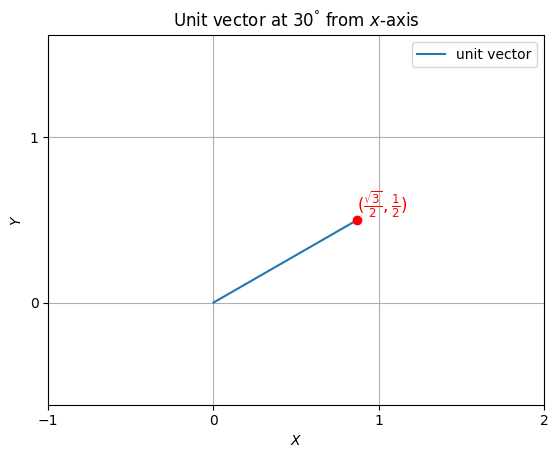
\includegraphics[width=\textwidth]{plots/plot.png}
	\end{figure}


  
\end{document}


